\subsection{}


\xdef\myAlpha{30}
\pgfmathparse{\myAlpha + 360}
\xdef\mySecondAlpha{\pgfmathresult}
\begin{center}
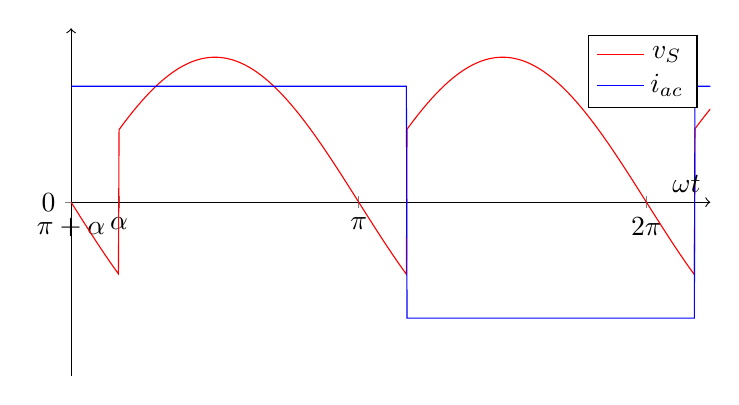
\begin{tikzpicture}
\begin{axis}[domain=0:400, 
             axis x line=middle, 
             axis y line=left, 
             xtick={\myAlpha,180,\mySecondAlpha,360}, 
             xticklabels={$\alpha$,$\pi$,$\pi+\alpha$,$2\pi$},
             ytick={0},
             yticklabels={0},
             x axis line style={->},
             xlabel={$\omega{}t$},
             xlabel style={align=right}, 
             y axis line style={->},
             width=0.8\textwidth,
             height=6cm,
             %width=\uncontrolledRectifierGraphWidth,
             ymax=1.2,
             ymin=-1.2,
             ] 
    \addplot[red, samples=1000] {sin(mod(180+x-\myAlpha,180)+\myAlpha)}; 
    \addplot[blue, samples=1000] {+0.8-1.6*and(1,mod(x-\myAlpha,360)>180)}; 
    \legend{$v_S$, $i_{ac}$}
\end{axis}
\end{tikzpicture}
\end{center}